\documentclass{article}
\twocolumn
\usepackage[T1]{fontenc}
\usepackage{amsmath}
\usepackage[a4paper, total={7in, 9in}]{geometry}
\usepackage{graphicx}
\graphicspath{ {./img/} }

\begin{document}

\section*{I. Introduction to Genetics}
\subsection*{A. Concept of Genes (chromosomes, genes, alleles, locus, karyotype, homozygous dominant and recessive, heterozygous)}
\subsubsection*{Chromosomes}
Chromosomes are structures within cells which contain genetic material in the form of DNA (deoxyribonucleic acid) in cells that are preparing to divide.


Basic Information
\begin{itemize}
    \item Each chromosome has one very long DNA molecule with hundreds or thousands of genes.
    \item Genes are the units of Inheritance
    \item Inherited DNA is what determines development
\end{itemize}


DNA Structure
\begin{itemize}
    \item Made up of two long chains called strands arranged in a double helix
    \item Each chain is made up of four kinds of chemical building blocks called nucleotides (A, T, C and G)
    \item the way DNA is organized is similar to how we arrange letters in the alphabet, (e.g. rat and tar are arranged differently with different meanings, but use the same letters)
\end{itemize}
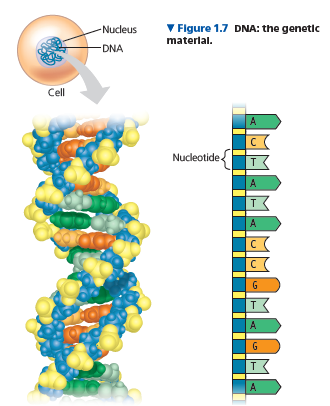
\includegraphics[scale=1.5]{dnahelixstructure.png}


\subsubsection*{Genes}
\begin{itemize}
    \item Provides the blueprint for making a protein, a gene can specify the building block for a specific protein/enzyme, or another gene can specify the building block for an antibody
    \item May also control protein production indirectly with RNA as an intermediary, transcribed into RNA and translated into amino acids.
    \item Amino acid chains forms a specific protein with a unique shape and function.
    \item How a gene directs the cellular product is called gene expression
    \item Genetic code sequences are all universal so one snippet in one chromosome would mean the same in another chromosome
\end{itemize}


Genome
\begin{itemize}
    \item The "library" of genetics
    \item The genomic sequence is the entire sequence of nucleotides
    \item Studied in genomics
\end{itemize}


\subsubsection*{Alleles}
These are the different version of Genes
\begin{itemize}
    \item Can create variations in the sexually reproducing population
    \item Is created during the crossing over in Prophase I
    \item Alleles can be e.g. (White and Purple color of flower)
    \item The two alleles form together from the sperm and egg cell
    \item The dominant allele takes the physical traits
\end{itemize}

\subsubsection*{Locus}
The locus is the location of a sepcific gene
\begin{itemize}
    \item plural is loci; from latin meaning place
    \item a gene could be in a specific locus, and the exact same type of gene (but maybe a different variation) could be found in a different chromosome of the same karyotype
    \item example: a gene with freckles can be in one locus, but in the other locus the gene says there is no freckles
    \item Represented twice in a diploid cell, once on each homolog of a specific pair of chromosomes
    \item Can be the same or different gene in a loci
\end{itemize}

\subsubsection*{Karyotype}
\begin{itemize}
    \item The order of chromosomes based on it's length
    \item There are 23 different types in 46 human chromosomes
\end{itemize}
\includegraphics*[scale=1.8]{karyotype.png}


\subsubsection*{Homozygous dominant and recessive}


Homozygous dominant and recessive
\begin{itemize}
    \item When there is two of the same allele which is genetically dominant/recessive in the same loci
    \item e.g (BB for both brown eyes)
    \item e.g (bb for both blue eyes)
\end{itemize}

Heterozygous
\begin{itemize}
    \item When there are two different alleles in the same loci, so one is dominant and one is recessive
    \item The recessive one is no longer shown
    \item e.g (Bb for brown eyes since the small b is disregarded)
\end{itemize}


\subsection*{B. Background information on Gregor Mendel and how he was able to come up with the three laws/principles of genetics}

\begin{itemize}
    \item Born 1823
    \item Augustinian monk who discovered the basic principles of heredity
    \item Started from breeding garden peas in experiements
    \item From Austria (part is currently in Czechia), and studied at tha Olmutz Philosophical Insitute
    \item Studied in the University of Vienna afterwards
    \item Started breeding garden peas in the abbey garden to study inheritance
    \item he noticed and coined heritable feature is called a character, while a variant is called a trait. (e.g. eye color is a character, while brown is a trait)
    
\end{itemize}
\subsection*{C. Construction of Punnett square of monohybrid and dihybrid crosses}

\begin{itemize}
    \item diagramtic device for predicting the allele composition of an offspring
    \item Individual genetic makeup is needed for this to be determined
    \item Denote the dominant allele as a capital letter and the recessive one with a lowercase letter
    \item The offspring when the alleles breed, there are different generations based on how many times it's crossed
\end{itemize}

\subsubsection*{Monohybrid Cross}
\begin{itemize}
    \item Only one item is being followed within the cross
    \item example: One trait only looks for the character of color
\end{itemize}

\subsubsection*{Dihybrid Cross}
\begin{itemize}
    \item This is when there is two independent variables which are tracked within the Cross
    \item example: When there is one trait for shape, and one trait for color
\end{itemize}
Example of a punnett square (place the first allele on the top row, and place the second allele on the left column and make the letters intersect based on the locations IDK IF THAT MAKES SENSE LOL)
\begin{center}
    \begin{tabular}{ c | c | c }
      & P & p \\ 
      \hline
     P & PP & Pp \\
     \hline  
     p & Pp & pp    
    \end{tabular}
\end{center}

\subsection*{D. Genotypic and Phenotypic Ratios}

\subsubsection*{Basic Defitions}
\begin{itemize}
    \item Genotype - This is the genetic makeup of the trait
    \item Phenotype - This is the physical characteristic of the trait
    \item The difference between a genotype and a phenotype is that when the allele is heterozygous it's genetic makeup would be Pp, but its pheonotype would still be dominant even though it's only 50\% dominant genotypically.
\end{itemize}
\subsubsection*{Generations}
\begin{itemize}
    \item P Generation: The original parents and the start of the crosses
    \item F1 Generation: First cross, 2 offspring total
    \item F2 Generation: Second Cross, 4 offspring total
\end{itemize}

\includegraphics*[scale=0.7]{generation.png}
P.S. I feel like reading section two would be better since it explains the dominance part more, but if you get dominance already feel free to read this part in full already. 
\subsubsection*{Genotypic ratios and punnet squares}
Now let us look at specific examples of punnet squares to look at it's respective genotypes and pheonotypes, and their respective ratios when breeding.

\begin{center}
    \begin{tabular}{ c | c |c }
      & P & P \\ 
      \hline
     P & PP & PP \\  
      \hline
     P & PP & PP    
    \end{tabular}
\end{center}

As we can observe in this table, when both of the alleles are identical, the genotypes of all of the offspring would be the same. This is called true breeding as they would only produce one characteristic of cell. Therefore the Phenotype would all be dominant, with a genotype of PP. The same would happen if only recessive alleles were bred 

\begin{center}
    \begin{tabular}{ c | c |c }
      & P & P \\ 
      \hline
     p & Pp & Pp \\  
      \hline
     p & Pp & Pp    
    \end{tabular}
\end{center}

Notice in this table when we breed PP and pp, the offspring are all Pp. This would mean that the geneotype is Pp, but the offspring would all be pheonotypically dominant.

\begin{center}
    \begin{tabular}{ c | c | c }
      & P & p \\ 
      \hline
     P & PP & Pp \\
     \hline  
     p & Pp & pp    
    \end{tabular}
\end{center}

Looking at the previous punnet square notice how given two heterozygous alleles, we are left with two homozygous alleles (one dominant and one recessive), and two heterozygous alleles. This gives a genotypic ratio of 1:2:1 where there is 1 part PP, 1 part pp, and 2 parts Pp, and a phenotypic ratio of 3:1, where 3 of the offspring shows the dominant trait and only 1 shoes the recessive trait.

\begin{center}
    \begin{tabular}{ c | c | c }
      & P & p \\ 
      \hline
     p & Pp & pp \\
     \hline  
     p & Pp & pp    
    \end{tabular}
\end{center}

Lastly, when we breed a Pp and pp allele, we are left with 2 Pp, and 2 pp. This gives a genotypic ratio of 1:1 Pp and pp, and a phenotypic ratio of 1:1 dominant and recessive traits.

\includegraphics*[scale=0.9]{square.png}
\break
\includegraphics*[scale=0.6]{square2.png}

Therefore: \break
\begin{itemize}
    \item When PP and PP or pp and pp, the pheonotypic ratio is 1, and the genotypic ratio is 1 (also true breeding)
    \item When PP and pp, the phenotypic ratio and genotypic ratio is 1
    \item When Pp and Pp, the phenotypic ratio is 3:1 and the genotypic ratio is 1:2:1
    \item When Pp and pp, the phenotypic and genotypic ratio is 1:1
    \item Additionally: In Dihyrbrid crosses of two Parents of different alleles the pheonotypic ratio is:
    \item F1 - 3:1 (3RRBB:1rrbb)
    \item F2 - 9:3:3:1 (9RR)
    \item While the genotypic ratio is
    \item F1 - 1:2:1 (RRBB,2RrBb,rrbb)
    \item F2 - 1 (RRBB, 2RRBb, 2RrBB, 4RrBb, 1RRbb, 2Rrbb, 1rrBB, 2 rrBb, 1 rrbb) basta that
\end{itemize}

\section*{II. Mendelian Genetics}
\subsection*{A. Law/Principle of Dominance}

\begin{itemize}
    \item The law of dominance is when there is one allele which dominates the other (Dominant and recessive genes)
    \item Exact Quote: "Some alleles are dominant while others are recessive. An organism with at least one dominant allele displays the effect irrespective of the prescence of the respective one."
    \item When we have a dominant and recsisive allele in the genotype (e.g. Pp), the dominant allele will display the effect irrespective of the recessive one
    \item Kind of like an if statement where if P >= 1 then, trait = dominant
    \item When both genes are dominant, then the gene will be dominant
\end{itemize}

\subsection*{B. Law/Principle of Independent Segregation}
\begin{itemize}
    \item During gamete formation, each alleles segregate from each other such that each gamete formed carries only one allele for each gene
    \item When we have an allele (e.g. CC these are split into C and C. It then combines with the other parent (e.g. cc) so each they would then combine with the other split gamete to make the new alleles)
    \item Easily understandable because of the knowledge of meiosis, but was introduced by mendal and made into a law.
\end{itemize}
\subsection*{C. Law/Principle of Independent Assortment}
Following the historical context of Mendelian Genetics, Mendel's statements first became principles when he published his works. Then, they become laws for some time. Then, when technology advanced, they were considered principles because the law/principle of dominance and independent assortment already had some limitations; hence, debunked as laws. 
\begin{itemize}
    \item Randomness within the human body.
    \item Although our body is organized, some process have no fixed patter. (e.g. alignment of chromosomes on the metaphase plate)
    \item In a cell undergoing meiosis, metaphase is where chromosomes align, but which cell the chromosomes go to are random.
    \item There is no guarantee where the alleles will end up when meiosis happens so the traits are independent to each other.
    \item Example: Given Aa, Bb, and Cc, you won't actually know where each gene will go during meiosis, so it can be ABc and abC or something else along those lines. 
    \item Dihybrid cross is needed to see how this works, as we need to look at two or more gene sets for the purpose of understanding the law
\end{itemize}

\section*{III. Non-Mendelian Genetics}
\subsection*{A. Incomplete Dominance}
\begin{itemize}
    \item Does not completely mask the recessive allele given it is heterozygous
    \item Given a flower with red and white colors where red is dominant, Rr would be color pink as it does not fully mask it
    \item Happens because the allele is not completely dominant to the recessive allele, and therefore a mixture of both happens
\end{itemize}\includegraphics*[scale=0.7]{codominance.png}

\subsection*{B. Codominance}
\begin{itemize}
    \item This is when there are two alleles which are shown in different parts of the cell.
    \item Easy to spot in animals that have more than one pigment color
    \item E.g. spotted cows, and petals with different colors
    \item Can also be seen in blood type like AB where AB is codominant with one another
\end{itemize}\includegraphics*[scale=0.7]{codeminance2.png}


\subsection*{C. Pleiotropy}
\subsubsection*{Definition}
\begin{itemize}
    \item pleion - more
    \item tropos - ways
    \item When a gene can have a various amount of traits, such as height, color and body shape
    \item introduced by Ludwig Plate
    \item When it is mutated in one specific trait of the gene, it could affect the other genes
\end{itemize}

\subsubsection*{Gene pleiotropy}
\begin{itemize}
    \item aka. molecular-gene pleiotropy, functions of the gene, and other factors impacted by said gene
\end{itemize}

\subsubsection*{Developmental pleiotropy}
\begin{itemize}
    \item Focuses on mutations and how one change influences multiple traits
    \item This is because one alteration affects other different traits
    \item Diseases related to pleiotropy generally come from deficiencies in multiple organs
\end{itemize}

\subsubsection*{Selectional pleiotropy}
\begin{itemize}
    \item How select components are affected by gene mutations
    \item How it can transfer its genes through sexual reproduction
    \item Only concered with the impact of natural selection on traits
\end{itemize}
\subsection*{D. Multiple Alleles}
\begin{itemize}
    \item Where there is many variations of a single gene
    \item In diploid organisms it can only express two alleles at the same time, they can be homozygous or heterozygous
    \item New alleles are created through spontatneous mutations, and the effect is a new sequence of DNA
    \item this mutation causes the amino acids to change, and its severity varies
    \item Focus on certain phenotypes created by certain Alleles, one phenotype can cause a large number of mutations.
    \item The mutation of alleles alone isn't necessarily good or bad as it is reliant on how that certain modification works with the entire system, so some varieties do better in specific conditions (e.g. skin tone variations based on where someone lives, notice how white people have white skin and live in colder areas whilst people from africa have darker skin)
\end{itemize}
\subsection*{E. Epistasis}
\begin{itemize}
    \item greek for "standing upon"
    \item The phenotypic expression is determined by another gene in a different locus
    \item There can be one allele which determines the color (e.g. black or brown)
    \item There can be another allele which determiness if the color will be followed (e.g. it can follow the given black or brown color, or disregard that allele and become gold)
\end{itemize}
\includegraphics*[scale=0.7]{epistasis.png}

\subsection*{F. Sex-linked Genes}
\begin{itemize}
    \item Men have X and Y Combination
    \item Female have X and X Combination
    \item Since there is only one X chromosome for men, it is more likely to have a recessive X trait be displayed, compared to women where the other X chromosome may be more dominant.
\end{itemize}
\subsubsection*{X-linked Genes}
\begin{itemize}
    \item 1098, X-linked genes: most are for something other than female anatomy, abnormal conditions such as hemophilia, Duchenne muscular dystrophy , fragile-X syndrome, some high blood pressure, congenital night blindness, G6PD deficiency, and the most common human genetic disorder, red-green color blindness.
    \item Responsible for male patterned baldnesss as well
    \item 800-900 protein-coding genes
    \item Due to having only one recessive gene, it is much easier to spread diseases for men as there is no dominant gene to cover it up. This is why autism is much more common for men compared to women as it is in the X chromosome (sir I based this on my own conclusions on a simple google search).
\end{itemize}
\subsubsection*{Y-linked Genes}
\begin{itemize}
    \item Much shorter and smaller compared to the X-Chromosomes
    \item about 26 genes and gene families.
    \item cell house-keeping activities (16 genes)
    \item sperm production (9 gene families) (sidenote: when any one of these genes are defective the infertility rate is much higher for men)
    \item SRY gene (Sex-determining Region of Y, for male anatomy, only one)
    \item Has evolved faster than the X chromosome and other chromosomes as the Y chromosome differs by 30\% compared to around 1-2\% overall.
    \item 60-78 protein-coding genes
\end{itemize}
\subsection*{G. Mitochondrial Inheritance}
\subsubsection*{Mitochondrial and chloroplast DNA}
\begin{itemize}
    \item Small circular copies which are present
    \item Thousands of copies within the mitochondrion
\end{itemize}
\subsubsection*{Inheritance}
\begin{itemize}
    \item High Copy Number - many within the cell
    \item Random Segregation - The copies are likely to end up in different cells through mitosis or meiosis because the mitochondrion has to pick a sidenote
    \item Single-parent inheritance - inherited from one parent only, for humans it is from the mother only (father took an L LOL)
\end{itemize}
\section*{IV. Pedigree Analysis}
\begin{itemize}
    \item Used to understand the inheritance of a trait, using a sort of "family tree" for genetics
    \item Proband is the person that initiates the pedigree.
    \item Used in predicting the likely mode of inheritance of certain a trait.
    \item All single gene controlled traits are now called Mendelian.
\end{itemize}
\includegraphics*[scale=0.7]{pedigree.png}

\subsection*{A. Autosomal Dominant (AD)}
\begin{itemize}
    \item When the trait is manifested in a heterozygous genotype
    \item Transmitted through either sex
    \item Does not skip generations (Pp always lives in one option or another if that makes sense)
\end{itemize}
\subsection*{B. Autosomal Recessive (AR)}
\begin{itemize}
    \item When the trait needs two of the recessive alleles for it to be manifested
    \item More likely in consan guineous marriages, where relatives mate as they have more similar genes
    \item 25\% chance between two heterozygous parents in a specific gene (refer to 1:3:1 ratio)
\end{itemize}
\subsection*{C. X-linked Dominant (XD)}
\begin{itemize}
    \item More common in females than males
    \item Does not skip generations
    \item Either parent can transmit the trait
    \item Mother has a 50\% chance of spreading a trait irrespective of sex 
    \item A male only inherits an X-linked dominant trait from their mother, and only passes it down to his daughters
    \item X-linked dominant disorders are relatively uncommon as compared to other
    Mendelian diseases.
\end{itemize}
\subsection*{D. X-linked Recessive (XR)}
\begin{itemize}
    \item Affects predominantly males from an asymptomatic mother
    \item Skips generations and is passed from the mother to son to grandaughter
    \item 50\% of sons are from a carrier mother, and 50\% are carrier daughters
    \item Never from father to son, as father passes down Y Chromosome instead of X (Think X from mom, Y from dad)
    \item All daughters of an affected man will be carriers if the mother is
    homozygous dominant.
\end{itemize}
\subsection*{E. Y-linked (Y)}
\begin{itemize}
    \item Holandric traits
    \item Passed from father to all sons if gene is located in the non recombining region
    \item Only males are affected
    \item Mutations are known to affect fertility
\end{itemize}
\end{document}